Diagrammatic notation for representing Slater determinants and operators originated with Richard Feynman in the field of quantum field theory (QFT). The methods were further developed for applications in many-body physics by, for example, Paldus and Cizek in 1975 \cite{Ref160}. The following will be a brief description of these diagrams. For a more thorough explanation of these diagrams, please refer to Chapter 4 of Ref. \cite{Ref21} and Ref. \cite{Ref160}.  

% Why Diagrammatic Methods
Diagrammatic methods are practical in studying many-body systems because the equations involved with solving these methods can get out of hand quickly. In addition, diagrammatic methods provide a more compact way to display these equations, which can hint at how specific components of the calculations will cancel or combine with other parts.

%% Fermi vacuum state and fundamental excitations

First, we will begin by representing the primary states in diagrammatic representation. First, the reference state is represented by nothing; for most systems in this thesis, the reference state will be the Fermi vacuum state ($|\Phi_0\rangle$). A one-particle one-hole excitation, $|\Phi^a_i \rangle$, is represented by two vertical lines. The line pointing upwards represents a state that is unoccupied in the Fermi vacuum state (i.e., indexed by $a$, $b$, $c$, ...), and a line pointing downwards represents a state that is occupied in the Fermi vacuum state (i.e., indexed by $i$, $j$, $k$, ...). Any line which does not have a directional arrow could represent either state (i.e., would be indexed with $p$, $q$, $r$, ...). Note that neither the horizontal arrangements nor spacing are significant in the representation. A two-particle, two-hole excited state, $| \Phi_{ij}^{ab} \rangle$, is represented by four vertical lines, two of which point down and two which point up. Following this pattern, an n-particle n-hole excited state is represented by 2n vertical lines, where n points upwards and n points downwards. Fig. \ref{fig:diagrams1} shows the diagrammatic representations of the Fermi vacuum state, the one-particle one-hole, and the two-particle two-hole excited states.

\begin{figure}
    \centering
    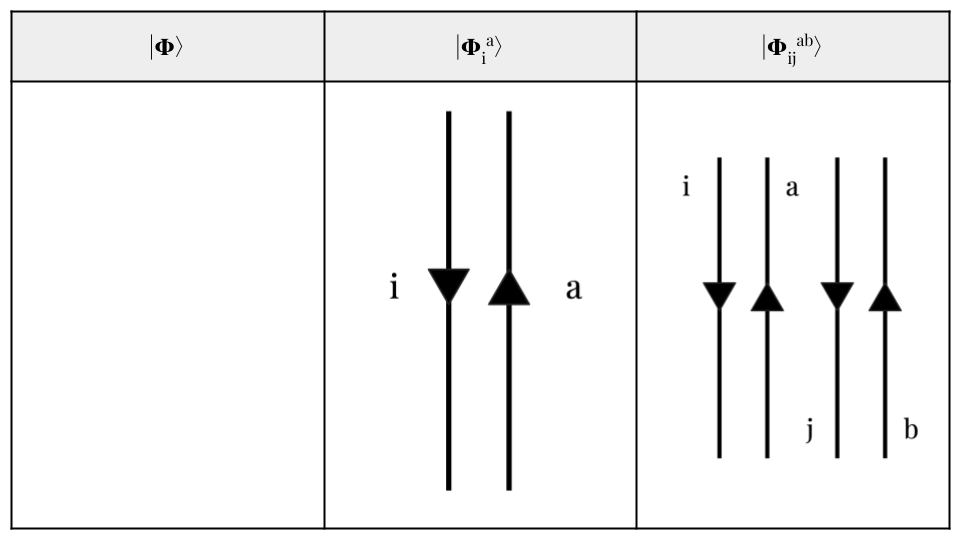
\includegraphics[scale=0.25]{Images/Chapter2/Diagrams_1.png}
    \caption{Diagrammatic representations for the Fermi vacuum state, the one-particle one-hole excited state, and the two-particle two-hole excited state.}
    \label{fig:diagrams1}
\end{figure}

Representing the excited states as creation and annihilation operators acting on the Fermi vacuum state is also possible. Remember that the one-particle one-hole excited state can be written as $|\Phi_i^a\rangle = a_a^\dagger a_i|\Phi_0\rangle$ where $a^\dagger$ is a fermionic creation operator and $a$ is the fermionic creation operator. This means that the two-particle two-hole excited state can be written as $|\Phi_{ij}^{ab}\rangle = a^\dagger_aa^\dagger_ba_ia_j|\Phi_0\rangle$.

The state $a_a^\dagger a_i|\Phi_0\rangle$ can be represented the same way as $|\Phi_i^a\rangle$, but with two horizontal lines at the bottom to represent the Fermi vacuum state. To represent the bra of this state ($\langle \Phi_i^a| = \langle \Phi_0|a^\dagger)_ia_a$ is represented in the same way, but the vertical lines representing the Fermi vacuum state are moved to the top. The two-particle two-hole excited state is represented similarly. These diagrams are shown in Fig. \ref{fig:diagrams2}.  Note that there is some ambiguity in the representation of $|\Phi_{ij}^{ab}\rangle$ in this representation, it could also represent $|\Phi_{ij}^{ba}\rangle$.

\begin{figure}
    \centering
    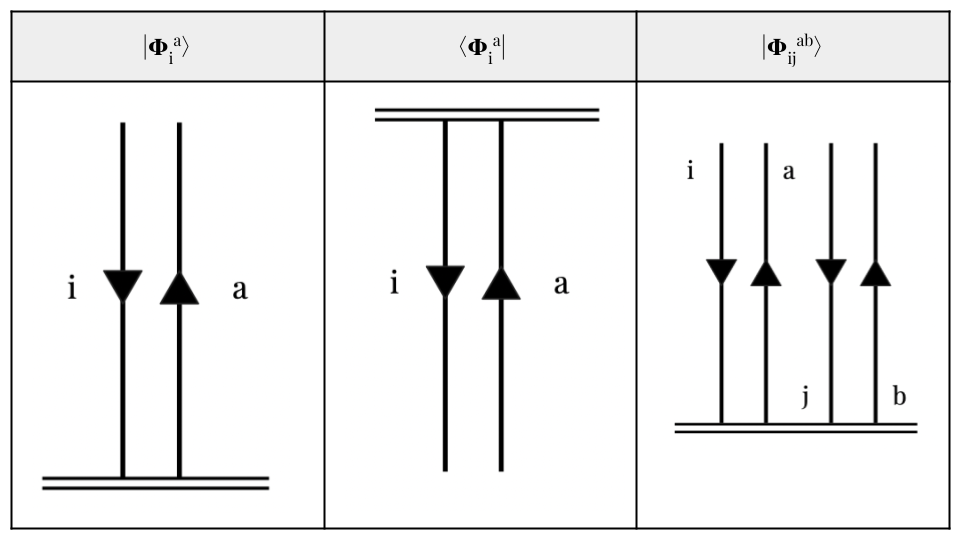
\includegraphics[scale=0.25]{Images/Chapter2/Diagrams_2.png}
    \caption{Diagrammatic representations for the one-particle one-hole and two-particle two-hole excited states written as annihilation and creation operators applied to the Fermi vacuum state.}
    \label{fig:diagrams2}
\end{figure}

%% Basic operator notation
Now that we have the diagrammatic notation for the various states, we can define a notation for the various operators. Here we will explicitly define the one-body and two-body operators in diagrammatic notation, but the form of the higher-order operators will follow the same patterns.

We can define a generic one-body operator as:

\begin{equation}
    \hat{O}_1 = \sum_{pq}\langle p | \hat{o}_1 | q \rangle \{a^\dagger_pa_q\},    
\end{equation}

where p and q can be occupied or unoccupied states, this one-body operator can be represented with either diagram in Fig. \ref{fig:one_body_generic}. The horizontal orientation of the lines does not matter so the lines can be in the purely vertical orientation, as in the left diagram, or they can be slanted, as in the right diagram. Since the lines in neither diagram of Fig. \ref{fig:one_body_generic} have directional arrows, the lines are represented by indices p and q.

\begin{figure}
    \centering
    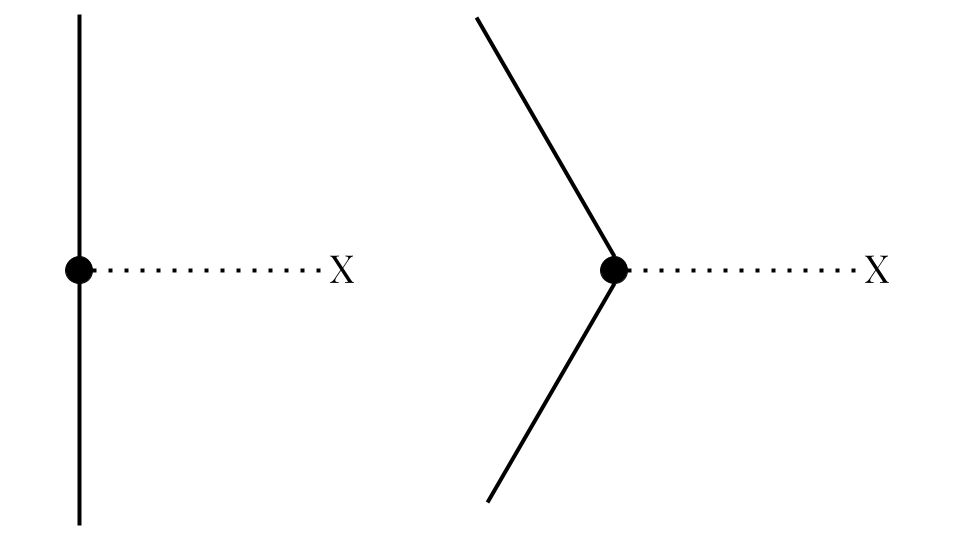
\includegraphics[scale=0.25]{Images/Chapter2/one_body_generic.png}
    \caption{A generic representation of the one body operator. The orientation of the lines does not matter, so the diagram can be represented with both lines being entirely vertical or with the lines being slanted. Since these lines do not have arrows, they represent generic single-particle states that could be occupied or unoccupied in the Fermi vacuum state.}
    \label{fig:one_body_generic}
\end{figure}

When creating the specific diagrams for the one-body operator, there are four options, as shown in Fig. \ref{fig:one_body_specific}.  There is one diagram where both indices are from states that are unoccupied in the Fermi vacuum state, which is represented by the top left diagram and equation form as:

\begin{equation}
    \sum_{ab} \langle a | \hat{o}_1 | b \rangle \{a^\dagger_aa_b\}.
\end{equation}

One diagram also results from having both states taken from the states occupied in the Fermi vacuum state. This is the diagram shown in the top right of Fig. \ref{fig:one_body_specific} and is represented in equation form as: 

\begin{equation}
    \sum_{ij} \langle i | \hat{o}_1 | j \rangle \{a^\dagger_ia_j\}.
\end{equation}

Finally, two diagrams can be created: one state is drawn from the occupied states and one from the unoccupied states. These are shown in the bottom row of Fig. \ref{fig:one_body_specific}. The bottom left diagram is represented in equation form:

\begin{equation}
    \sum_{ia} \langle a | \hat{o}_1 | i \rangle \{a^\dagger_aa_i\},
\end{equation}

the bottom right diagram in equation form is:

\begin{equation}
    \sum_{ia} \langle i | \hat{o}_1 | a \rangle \{a^\dagger_ia_a\}.
\end{equation}

\begin{figure}
    \centering
    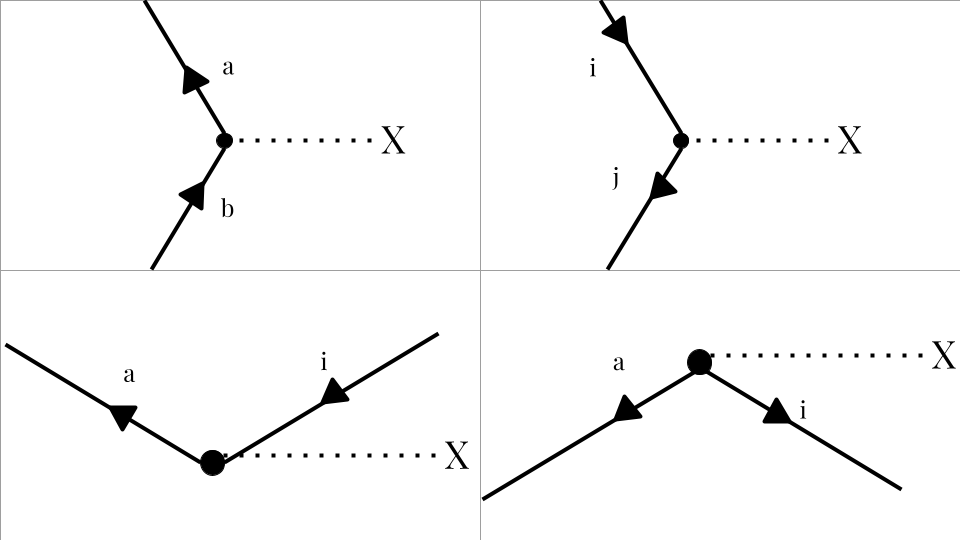
\includegraphics[scale=0.5]{Images/Chapter2/one_body_specific.png}
    \caption{The specific diagrams for the one-body operator, with the top left diagram for two unoccupied states, the top right diagram for two unoccupied states, and the bottom two diagrams containing one occupied and one unoccupied state.}
    \label{fig:one_body_specific}
\end{figure}

In the diagrams, the summation of the indices is implied using Einstein notation. In general, when creating diagrams from an equation, the index in the bra of the matrix element will exit the interaction vertex, and the index in the ket will be the line that enters the interaction vertex: $\langle left\ line | \hat{o}_1 | right\ line \rangle$.  

Finally, in this section, we can move onto the diagrammatic representation of a generic two-body operator, which we can represent in equation form as:

\begin{equation}
    \hat{O}_2 = \sum_{pqrs}\langle pq | \hat{o}_2 | rs \rangle \{a^\dagger_pa^\dagger_qa_sa_r\}.
\end{equation}

The generic two-body diagram can be described in Fig. \ref{fig:two_body_general}, and the nine specific two-body diagrams can be found in Fig. \ref{fig:two_body_specific}.

\begin{figure}
    \centering
    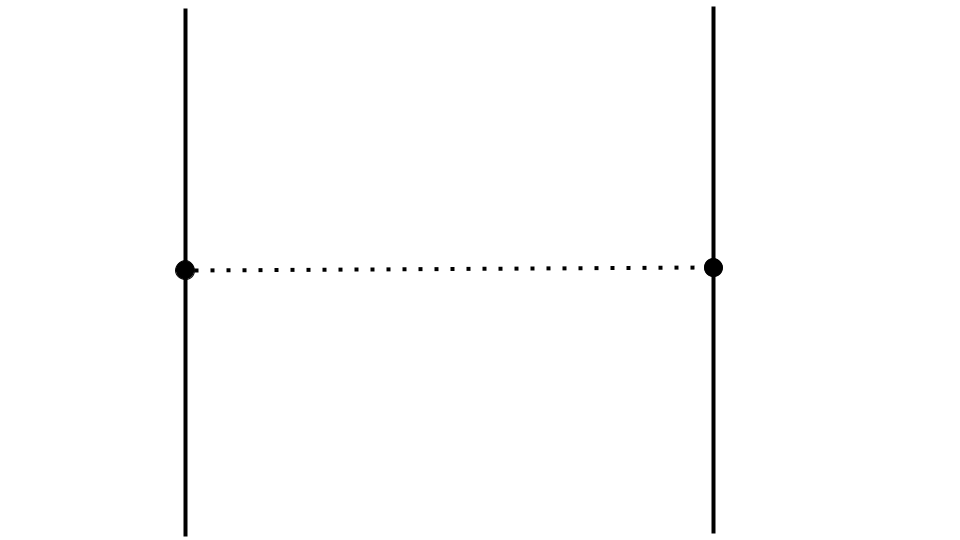
\includegraphics[scale=0.25]{Images/Chapter2/two_body_generic.png}
    \caption{The general diagram for a two-body interaction.}
    \label{fig:two_body_general}
\end{figure}

\begin{figure}
    \centering
    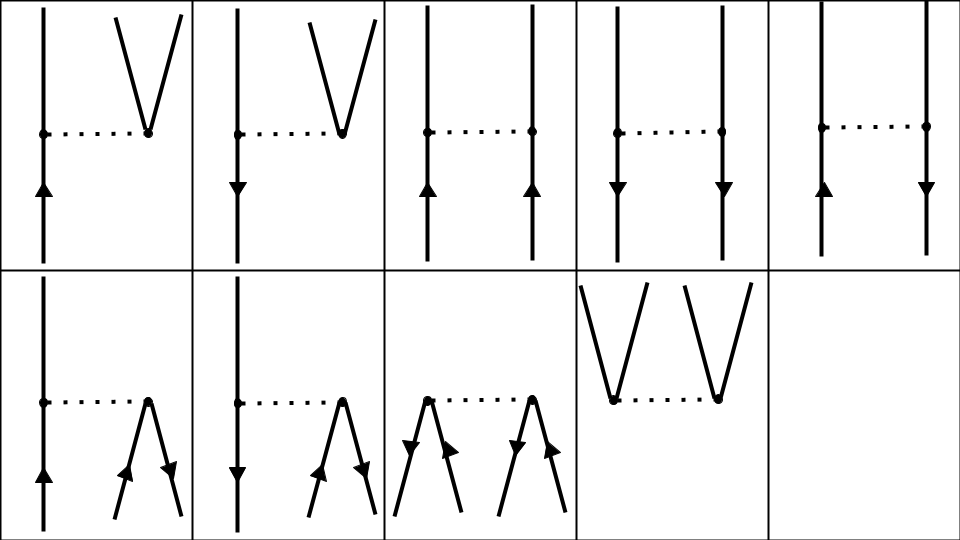
\includegraphics[scale=0.25]{Images/Chapter2/two_body_specific.png}
    \caption{The nine specific diagrams for a two-body interaction.}
    \label{fig:two_body_specific}
\end{figure}

From these examples, we can begin to create a set of rules for creating these diagrams and converting them to algebraic expressions:

\begin{enumerate}
    \item Lines representing occupied states in the Fermi vacuum are labeled with indices like $i$, $j$, $k$, ... and point downwards. Lines representing unoccupied states in the Fermi vacuum are labeled with indices $a$, $b$, $c$, ... and point upwards. Finally, lines that could represent either type of state are labeled with indices $p$, $q$, $r$, ... and have no directional arrows.
    \item The horizontal arrangement and spacing of the diagrams do not matter.
    \item Lines that represent the bra of the interaction matrix element leave an interaction vertex and are called external lines.
    \item Lines that represent the ket of the interaction matrix element enter an interaction vertex and are called internal lines.
    \item Every one body interaction vertex represents the factor $\langle out | \hat{o}_1 | in \rangle$.
    \item Every two-body interaction vertex represents the factor $\langle left-out\ right-out | \hat{o}_2 | left-in\ right-in \rangle$.
    \item If two lines start and end in the exact location, they are considered equivalent. Each set of equivalent lines in a diagram represents a factor of 1/2.
    \item The sign of a diagram is calculated using $(-1)^{(n_{occ} + l)}$, where $n_{occ}$ are the number of lines representing states that are occupied in the Fermi vacuum state and l is the number of loops in the diagram.
    \item Each pair of unique external lines (i.e., the bras of the interactions) that are not connected to the same interaction picks up a permutation factor.
\end{enumerate}